\documentclass[11pt]{article}
\usepackage{amsmath,amssymb,amsmath,amsthm,amsfonts}
\usepackage{latexsym,graphicx}
\usepackage{fullpage,color}
\usepackage{url,hyperref}
\usepackage{natbib}
\usepackage{graphicx,subfigure}
\usepackage{algorithm}
\usepackage{algorithmic}
\usepackage{listings}
\usepackage{xcolor}
\usepackage{color}

\numberwithin{equation}{section}

\pagestyle{plain}

\setlength{\oddsidemargin}{0in}
\setlength{\topmargin}{0in}
\setlength{\textwidth}{6.5in}
\setlength{\textheight}{8.5in}

\newtheorem{fact}{Fact}[section]
\newtheorem{question}{Question}[section]
\newtheorem{lemma}{Lemma}[section]
\newtheorem{theorem}[lemma]{Theorem}
\newtheorem{assumption}[lemma]{Assumption}
\newtheorem{corollary}[lemma]{Corollary}
\newtheorem{prop}[lemma]{Proposition}
\newtheorem{claim}{Claim}[section]
\newtheorem{remark}{Remark}[section]
\newtheorem{definition}{Definition}[section]
\newtheorem{prob}{Problem}[section]
\newtheorem{conjecture}{Conjecture}[section]
\newtheorem{property}{Property}[section]

\def\A{{\bf A}}
\def\a{{\bf a}}
\def\B{{\bf B}}
\def\bb{{\bf b}}
\def\C{{\bf C}}
\def\c{{\bf c}}
\def\D{{\bf D}}
\def\d{{\bf d}}
\def\E{{\bf E}}
\def\e{{\bf e}}
\def\F{{\bf F}}
\def\f{{\bf f}}
\def\g{{\bf g}}
\def\h{{\bf h}}
\def\G{{\bf G}}
\def\H{{\bf H}}
\def\I{{\bf I}}
\def\K{{\bf K}}
\def\k{{\bf k}}
\def\LL{{\bf L}}
\def\M{{\bf M}}
\def\m{{\bf m}}
\def\N{{\bf N}}
\def\n{{\bf n}}
\def\PP{{\bf P}}
\def\Q{{\bf Q}}
\def\q{{\bf q}}
\def\R{{\bf R}}
\def\rr{{\bf r}}
\def\S{{\bf S}}
\def\s{{\bf s}}
\def\T{{\bf T}}
\def\tt{{\bf t}}
\def\U{{\bf U}}
\def\u{{\bf u}}
\def\V{{\bf V}}
\def\v{{\bf v}}
\def\W{{\bf W}}
\def\w{{\bf w}}
\def\X{{\bf X}}
\def\x{{\bf x}}
\def\Y{{\bf Y}}
\def\y{{\bf y}}
\def\Z{{\bf Z}}
\def\z{{\bf z}}
\def\0{{\bf 0}}
\def\1{{\bf 1}}



\def\AM{{\mathcal A}}
\def\CM{{\mathcal C}}
\def\DM{{\mathcal D}}
\def\EM{{\mathcal E}}
\def\GM{{\mathcal G}}
\def\FM{{\mathcal F}}
\def\IM{{\mathcal I}}
\def\JM{{\mathcal J}}
\def\KM{{\mathcal K}}
\def\LM{{\mathcal L}}
\def\NM{{\mathcal N}}
\def\OM{{\mathcal O}}
\def\PM{{\mathcal P}}
\def\SM{{\mathcal S}}
\def\TM{{\mathcal T}}
\def\UM{{\mathcal U}}
\def\VM{{\mathcal V}}
\def\WM{{\mathcal W}}
\def\XM{{\mathcal X}}
\def\YM{{\mathcal Y}}
\def\RB{{\mathbb R}}
\def\RBmn{{\RB^{m\times n}}}
\def\EB{{\mathbb E}}
\def\PB{{\mathbb P}}


\def\alp{\mbox{\boldmath$\alpha$\unboldmath}}
\def\bet{\mbox{\boldmath$\beta$\unboldmath}}
\def\epsi{\mbox{\boldmath$\epsilon$\unboldmath}}
\def\etab{\mbox{\boldmath$\eta$\unboldmath}}
\def\ph{\mbox{\boldmath$\phi$\unboldmath}}
\def\pii{\mbox{\boldmath$\pi$\unboldmath}}
\def\Ph{\mbox{\boldmath$\Phi$\unboldmath}}
\def\Ps{\mbox{\boldmath$\Psi$\unboldmath}}
\def\ps{\mbox{\boldmath$\psi$\unboldmath}}
\def\tha{\mbox{\boldmath$\theta$\unboldmath}}
\def\Tha{\mbox{\boldmath$\Theta$\unboldmath}}
\def\muu{\mbox{\boldmath$\mu$\unboldmath}}
\def\Si{\mbox{\boldmath$\Sigma$\unboldmath}}
\def\si{\mbox{\boldmath$\sigma$\unboldmath}}
\def\Gam{\mbox{\boldmath$\Gamma$\unboldmath}}
\def\Lam{\mbox{\boldmath$\Lambda$\unboldmath}}
\def\De{\mbox{\boldmath$\Delta$\unboldmath}}
\def\Ome{\mbox{\boldmath$\Omega$\unboldmath}}
\def\Pii{\mbox{\boldmath$\Pi$\unboldmath}}
\def\varepsi{\mbox{\boldmath$\varepsilon$\unboldmath}}

\def\argmax{\mathop{\rm argmax}}
\def\argmin{\mathop{\rm argmin}}
\def\bias{\mathsf{bias}}
\def\var{\mathsf{var}}
\def\sgn{\mathsf{sgn}}
\def\tr{\mathsf{tr}}
\def\rk{\mathrm{rank}}
\def\poly{\mathrm{poly}}
\def\diag{\mathsf{diag}}
\def\st{\mathsf{s.t.}}

\newcommand{\red}[1]{{\color{red}#1}}



\lstset{ %
extendedchars=false,            % Shutdown no-ASCII compatible
language=Python,                % choose the language of the code
xleftmargin=1em,
xrightmargin=1em,
basicstyle=\footnotesize,    % the size of the fonts that are used for the code
tabsize=3,                            % sets default tabsize to 3 spaces
numbers=left,                   % where to put the line-numbers
numberstyle=\tiny,              % the size of the fonts that are used for the line-numbers
stepnumber=1,                   % the step between two line-numbers. If it's 1 each line
                                % will be numbered
numbersep=5pt,                  % how far the line-numbers are from the code   %
keywordstyle=\color[rgb]{0,0,1},                % keywords
commentstyle=\color[rgb]{0.133,0.545,0.133},    % comments
stringstyle=\color[rgb]{0.627,0.126,0.941},      % strings
backgroundcolor=\color{white}, % choose the background color. You must add \usepackage{color}
showspaces=false,               % show spaces adding particular underscores
showstringspaces=false,         % underline spaces within strings
showtabs=false,                 % show tabs within strings adding particular underscores
frame=single,                 % adds a frame around the code
%captionpos=b,                   % sets the caption-position to bottom
breaklines=true,                % sets automatic line breaking
breakatwhitespace=false,        % sets if automatic breaks should only happen at whitespace
%title=\lstname,                 % show the filename of files included with \lstinputlisting;
%                                % also try caption instead of title
mathescape=true,escapechar=?    % escape to latex with ?..?
escapeinside={\%*}{*)},         % if you want to add a comment within your code
%columns=fixed,                  % nice spacing
%morestring=[m]',                % strings
%morekeywords={%,...},%          % if you want to add more keywords to the set
%    break,case,catch,continue,elseif,else,end,for,function,global,%
%    if,otherwise,persistent,return,switch,try,while,...},%
}


\begin{document}


\title{CS583A: Course Project}

\author{Name 1, Name 2, and Name 3}

%\date{ }

\maketitle




\section{Summary}

[Problem descriptions:] We pariticipe an active (or inactive with late submission) competition of classifying cats and dogs based on photos. 
[Methodology:] The final model we choose is ResNet50, a deep convolutional neural network architecture, which takes $256\times 256$ images as input and outputs the class labels.
[Implementation:] We implement the convolutional neural network using Keras (or we directly use the ResNet50 provided by Keras) and run the code on a MacBook Pro with one Intel i7 CPU and 32 GB memory (or a workstation with 4 NVIDIA GeForce XXX GPUs.)
[Evaluation metric:] Performance is evaluated on the classification accuracy.
[Score and ranking:] In the public leaderboard, our score is $0.95123$; we rank 79 among the 215 teams. In the private leaderboard, our score is $0.95234$; we rank 82 among the 217 teams. (Or, the result on the public leaderboard is not available until Month Day Year.)

(Note: In your report, remove the words in brackets.)


\section{Problem Description}



\paragraph{Problem.}
The problem is to classify cats and dogs based on photos.
This is a binary classification and image recognition problem.
The competition is at \url{https://www.kaggle.com/c/dogs-vs-cats}.
[Use your own words to give a very short description. Do NOT copy the description on Kaggle.]



\paragraph{Data.} 
The data are $256\times 256$ JPEG images.
The number of training samples is $n=25,000$.
The number of classes is $2$.
The training set is well-balanced: $n_{\textrm{dog}} = 12,500$ and $n_{\textrm{cat}} = 12,500$.


\paragraph{Challenges.}
[What makes the problem challenge? E.g., the training set is too small, the data is imbalanced, etc.]





\section{Solution}

\paragraph{Model.}
The model we finally choose is the ResNet50 \cite{he2016deep}, a standard deep convolutional neural network.
A description of ResNet is online: \url{https://en.wikipedia.org/wiki/Residential_network}.
[Describe your model only if it is non-standard.]


\paragraph{Implementation.}
We implement the ResNet50 model using Keras with TensorFlow as the backend. [Or, we directly use the ResNet model provided by Keras.]
Our code is available at \url{https://github.com/wangshusen/CS583A-2019Spring/}.
We run the code on a MacBook Pro with one Intel i7 CPU and 32 GB memory (or a workstation with 4 NVIDIA GeForce XXX GPUs.)
It takes $2.2$ hours to train the model.


\paragraph{Settings.}
The loss function is categorical cross-entropy.
The opitmizer is RMSprop.
[Specify the other hyperparameters such as learning rate, regularization, epochs, batch size, etc.]


\paragraph{Advanced tricks.}
[If you used advanced tricks, e.g., pretrain the model on ImageNet and fine-tune it on the Dog-VS-Cat dataset, then write down your tricks and discuss their contribution to the performance, e.g., improve the validation error by $5.6\%$.]

\paragraph{Cross-validation.}
We tune the parameters using a 5-fold cross-validation. [If you do not have GPU, you can simply partition the training data to 80\%-20\% or 90\%-10\% for hyperparameter tuning.]
[Just show the results of your final chosen model.]
Figure~\ref{fig:convergence} plots the the convergence curves on 80\% training data and 20\% validation data. [If you use 5-fold cross-validation, just plot one of the five folds.]
[Analyze the convergence curves. E.g., if the training accuracy is much better than the validation accuracy, then the model is likely to overfit the data, and that is why you pretrain your model on ImageNet.] 


%---------------------------------Figure---------------------------------%
\begin{figure}
	\begin{center}
		\subfigure[The classification accuracy on the training set and validation set.]{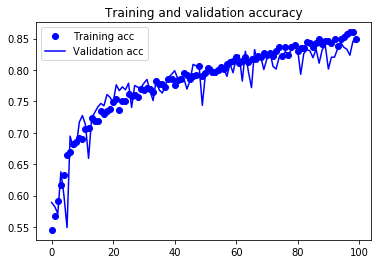
\includegraphics[width=0.48\textwidth]{acc.png}}
		\subfigure[The loss on the training set and validation set.]{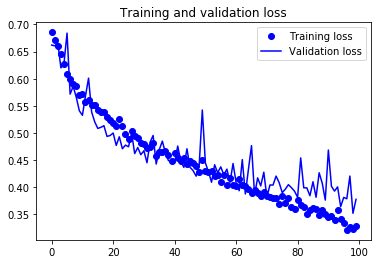
\includegraphics[width=0.48\textwidth]{loss.png}}
	\end{center}
	\caption{The convergence curves.}
	\label{fig:convergence}
\end{figure}
%---------------------------------Figure---------------------------------%





\section{Compared Methods}


[Try different methods (with brief descriptions) and report their performance.]



\section{Outcome}


We participated in an active competition.
Our score is 0.89311 in the public leaderboard and 0.90112 in the private leaderboard.
We rank 100/312 in the public leaderboard and 101/312 in the private leaderboard.
The screenshots are in Figure~\ref{fig:leaderboard}.





%---------------------------------Figure---------------------------------%
\begin{figure}
	\begin{center}
		\subfigure[Private leaderboard.]{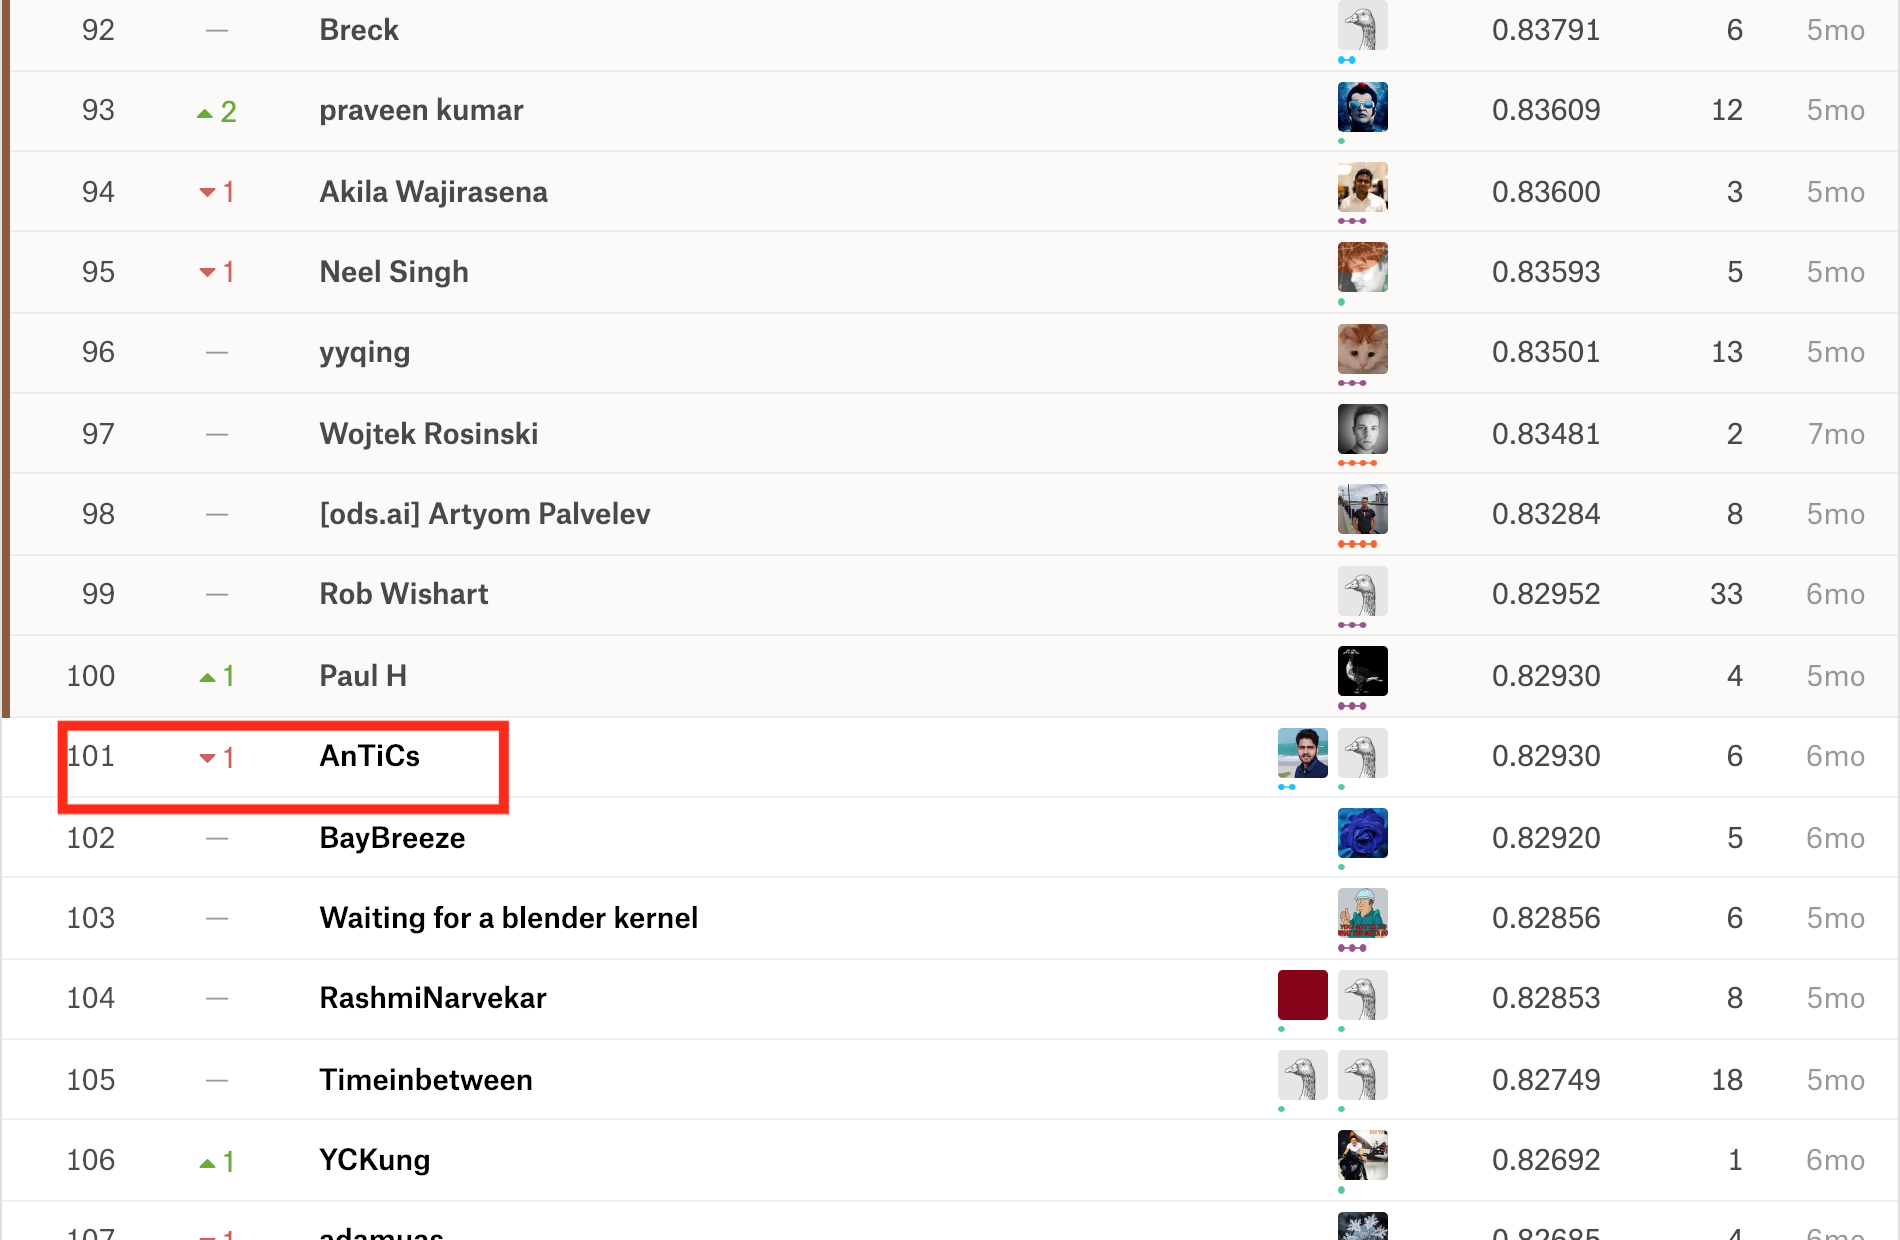
\includegraphics[width=0.48\textwidth]{private.png}}
		\subfigure[Public leaderboard.]{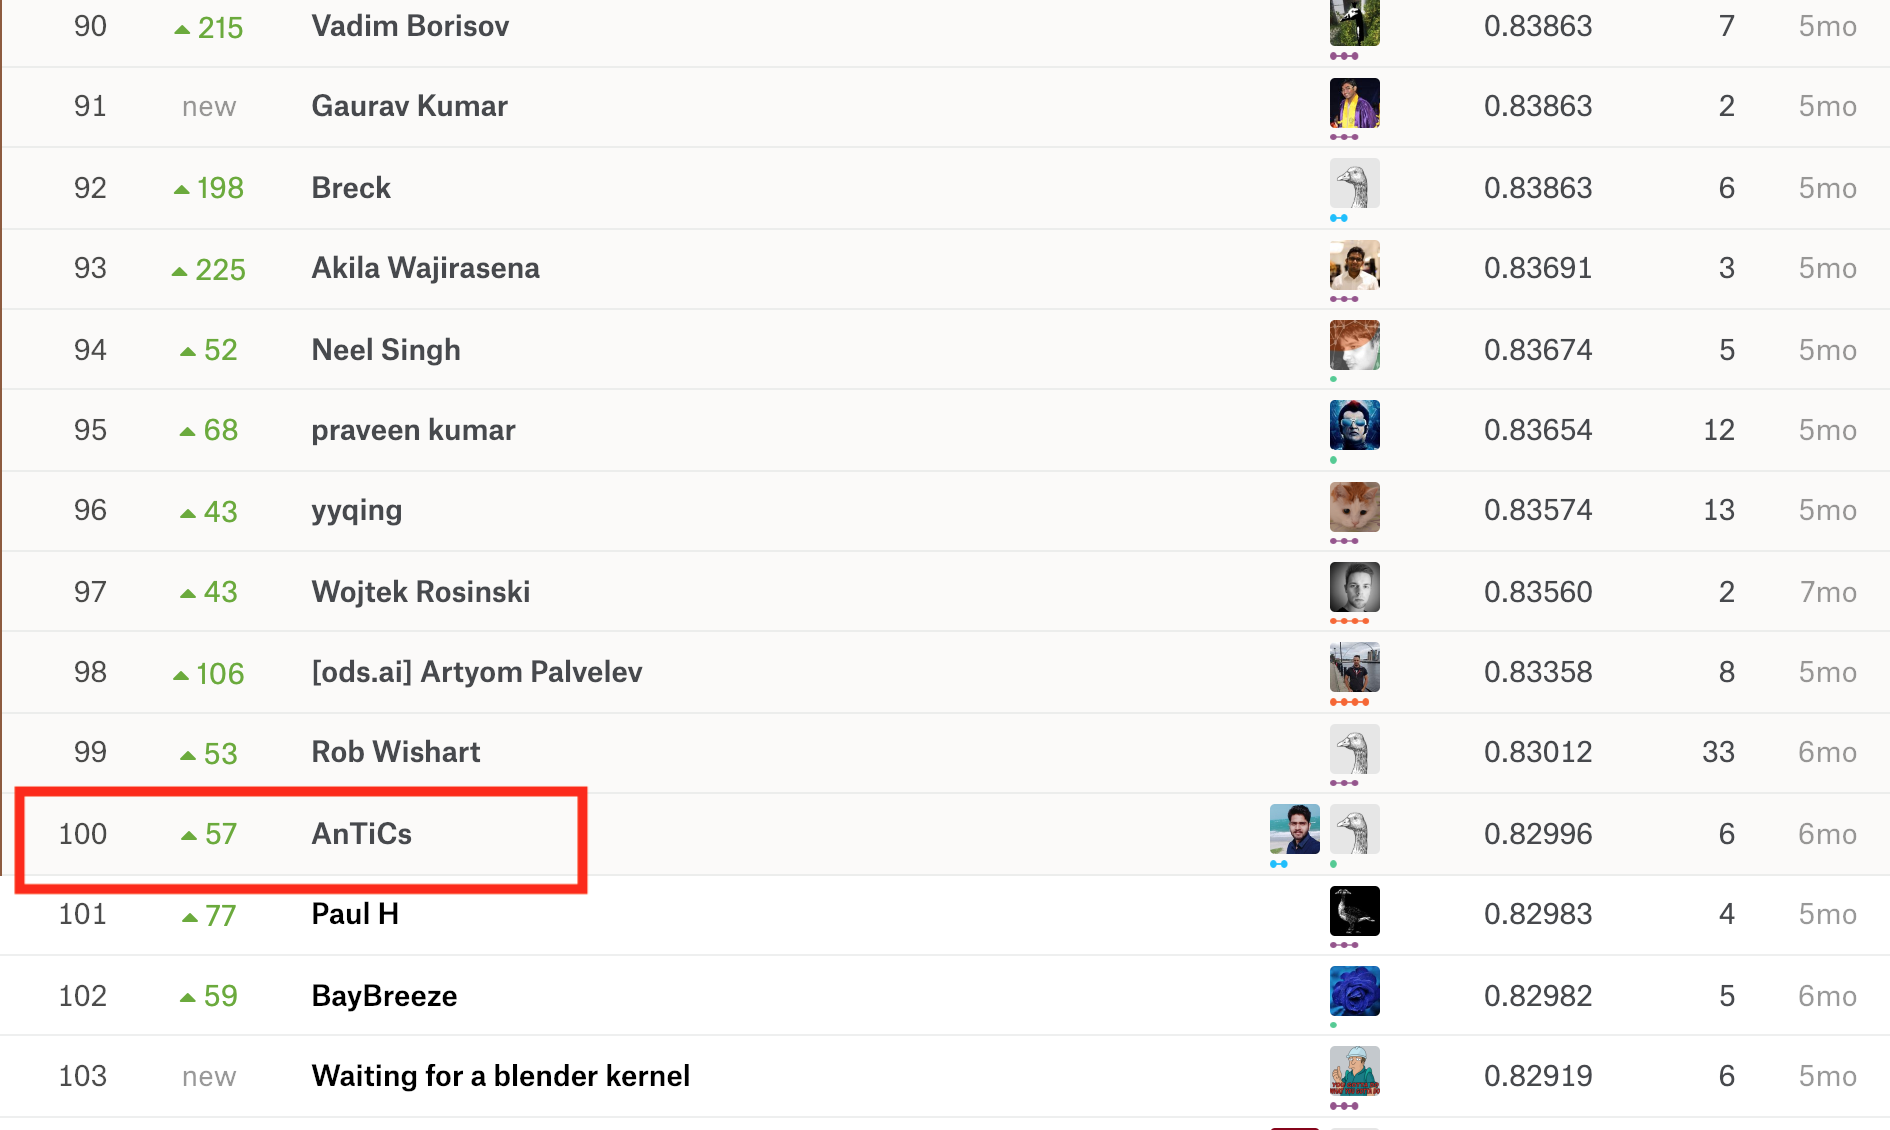
\includegraphics[width=0.48\textwidth]{public.png}}
	\end{center}
	\caption{Our rankings in the leaderboard.}
	\label{fig:leaderboard}
\end{figure}
%---------------------------------Figure---------------------------------%



%\vspace{3mm}
%\begin{lstlisting}
%import numpy
%
%def rfm(x, s, sigma):
%	n, d = x.shape
%	a = numpy.random.standard_normal((d, s)) / sigma
%	b = numpy.random.rand(1, s) * (2 * numpy.pi)
%	c = numpy.dot(x, a) + b
%	h = numpy.cos(c) * numpy.sqrt(2/s)
%	return h
%\end{lstlisting}
%\vspace{3mm}

%\newpage
\bibliographystyle{plain}
\bibliography{reference}


\end{document}
